\documentclass[12pt]{article}
\usepackage[a4paper,margin=2.5cm]{geometry}
\usepackage{graphicx}
\usepackage{setspace}
\usepackage{tikz}
\usepackage[spanish]{babel}
\usepackage[T1]{fontenc}
\usepackage{lmodern}
\usepackage{amsmath}
\usepackage{hyperref}
\usepackage{float}
\usepackage{ragged2e}

\begin{document}
\thispagestyle{empty}

% ---------- CARÁTULA ----------
\thispagestyle{empty}
\begin{center}
    \vspace*{\fill}

    {\Large \textbf{Universidad de San Andrés}}\\[0.8cm]
    {\Huge \textbf{Inferencia y Estimación}}\\[0.6cm]
    {\LARGE \textbf{Trabajo Práctico N.º 1}}\\[1.5cm]
    
    \begin{tikzpicture}
      \node[draw, rounded corners=6pt, inner sep=14pt, line width=0.8pt]
      {
        \begin{minipage}{0.78\textwidth}
          \begin{center}
            {\Large \textbf{Compresión de Imágenes}}\\[0.8cm]
            {\large \textbf{Profesores:} Matías Perlin, Pau García Gulisano, Juan Ponce}\\[0.4cm]
          \end{center}
        \end{minipage}
      };
    \end{tikzpicture}

    \vspace{1.2cm}

    {\large \textbf{Integrantes (Grupo 4):}}\\[0.4cm]
    {\large Máximo Barral - barralm@udesa.edu.ar - Legajo 36585}\\[0.2cm]
    {\large Lautaro Valentín Caminoa - lcaminoa@udesa.edu.ar - Legajo 36571}\\[0.2cm]
    {\large Franco Sandri - fsandri@udesa.edu.ar - Legajo 36530}\\[1.4cm]

    % ---------- RESUMEN ----------
    \section*{\small Resumen}
    \begin{justify}
    \small
    El presente trabajo aborda la compresión de imágenes mediante el análisis de componentes principales (PCA), una técnica estadística de reducción de dimensionalidad. Se estudió en primer lugar la correlación espacial entre píxeles vecinos, mostrando que una mayor redundancia local facilita la compresión. Posteriormente se implementó el algoritmo de PCA desde cero, segmentando las imágenes en bloques y proyectando los datos en un subespacio de menor dimensión, con el objetivo de evaluar la pérdida de información frente al ahorro de espacio. La reconstrucción de las imágenes evidenció que es posible mantener una alta fidelidad visual conservando solo una fracción de los componentes principales, aunque con pérdidas graduales en detalles finos al incrementar el porcentaje de compresión. Finalmente, el análisis cuantitativo mediante el error cuadrático medio (MSE) confirmó el compromiso entre eficiencia y calidad, validando a PCA como una herramienta efectiva para la compresión de imágenes en contextos donde la redundancia espacial es significativa.
    \end{justify}

    \vspace*{\fill}
\end{center}
\newpage

% ---------- NUMERACIÓN DE PÁGINA ----------
\setcounter{page}{1}    % comienza numeración en 1
\pagestyle{plain}       % Número centrado

% ---------- INTRODUCCIÓN ----------
\section{Introducción}

En épocas de \textit{big data}, el volumen de información generada y almacenada crece a un ritmo exponencial. Dentro de este escenario, la compresión de información (y en particular de imágenes) se convierte en un proceso esencial para optimizar el almacenamiento, reducir costos de transmisión y mejorar la eficiencia en el procesamiento de grandes volúmenes de información visual. El \textit{análisis de componentes principales} (PCA, por sus siglas en inglés) constituye una de las técnicas más utilizadas para la reducción de dimensionalidad.
\par\vspace{0.4cm}
El fundamento de PCA radica en identificar las direcciones de mayor varianza dentro de un conjunto de datos y proyectarlos en un subespacio de menor dimensión, sin perder información esencial. En la práctica, se implementa de manera eficiente a través de la \textit{Descomposición en Valores Singulares} (SVD). 

Sea $A \in \mathbb{R}^{n \times m}$ la matriz de datos centrados en la media. Su factorización SVD es:
\begin{equation}
A \;=\; U S V^\top,
\label{eq:svd}
\end{equation}
donde $U \in \mathbb{R}^{n \times n}$ y $V \in \mathbb{R}^{m \times m}$ son matrices ortogonales, y $S \in \mathbb{R}^{n \times m}$ es una matriz diagonal rectangular cuyos elementos $s_i \geq 0$ son los valores singulares de $A$.

Matemáticamente, consideramos que cada bloque de la imagen puede representarse como un vector $X \in \mathbb{R}^{m}$, donde $m$ corresponde al número de píxeles del bloque. A partir de ello, se construye la matriz de covarianza
\begin{equation}
\widehat{C_X} \;=\; \frac{1}{n-1}X^TX ,
\label{eq:covarianza}
\end{equation}
cuyos autovectores definen la base ortogonal de proyección. La transformación PCA consiste en proyectar los datos centrados en la media sobre los $k$ autovectores asociados a los mayores autovalores:
\begin{equation}
Y \;=\; V_k^\top (X - \mu_X),
\label{eq:proyeccion}
\end{equation}
mientras que la reconstrucción de los datos comprimidos se realiza aplicando la transformación inversa:
\begin{equation}
\widehat{X} \;=\; V_k Y + \mu_X.
\label{eq:reconstruccion}
\end{equation}

\par\vspace{0.4cm}

Existe una relación directa entre los valores singulares de $A$ y los autovalores de la covarianza $C_X$: 
\begin{equation}
\lambda_i \;=\; \frac{s_i^2}{n-1}, \quad i=1,\dots,m,
\label{eq:relacion-svd}
\end{equation}
de modo que los autovectores de $C_X$ coinciden con las columnas de $V$. Esta equivalencia asegura que PCA puede resolverse directamente mediante SVD, con ventajas de estabilidad numérica y eficiencia computacional.

\par\vspace{0.4cm}
Una vez obtenida la representación comprimida, surge la necesidad de evaluar su calidad respecto de la imagen original. Para ello se emplean métricas cuantitativas, siendo el error cuadrático medio (MSE) una de las más utilizadas:
\begin{equation}
\mathrm{MSE} \;=\; \frac{1}{N_w N_h}\sum_{i=1}^{N_w}\sum_{j=1}^{N_h}\big(p_{ij}-\widehat{p}_{ij}\big)^2,
\label{eq:mse}
\end{equation}
donde $N_w$ y $N_h$ son las dimensiones de la imagen y $p_{ij}$, $\widehat{p}_{ij}$ representan respectivamente los valores de los píxeles originales y reconstruidos. A su vez, el nivel de compresión alcanzado se cuantifica a través del porcentaje de espacio ahorrado:
\begin{equation}
S \;=\; \left(1-\frac{k}{m}\right)\times 100\%.
\label{eq:ahorro}
\end{equation}

El objetivo del presente trabajo es implementar PCA en el contexto de compresión de imágenes, evaluar su desempeño mediante métricas cuantitativas y estudiar la relación entre la correlación espacial de los píxeles y la eficiencia de la compresión. Con ello, se busca profundizar tanto en la comprensión teórica del algoritmo como en su aplicación práctica en el análisis moderno de datos visuales.

% ---------- METODOLOGÍA ----------
\section{Metodología}

En la primera etapa del trabajo se estudió la correlación entre píxeles vecinos de dos imágenes distintas. Para ello se construyeron pares de valores correspondientes a píxeles contiguos en dirección vertical, que luego fueron representados en gráficos de dispersión. Las distribuciones obtenidas evidenciaron que las imágenes no se comportan como conjuntos aleatorios de intensidades, sino que presentan una marcada relación entre valores cercanos. Esta observación se cuantificó mediante el cálculo de coeficientes de correlación de Pearson y, a continuación, se aplicó una transformación lineal que permitió desacoplar las variables y generar un nuevo sistema de ejes con componentes menos correlacionadas. Dicho procedimiento puso de manifiesto la capacidad de PCA para concentrar la variabilidad en una única dirección predominante, justificando así su utilización como técnica de reducción de dimensión.

Posteriormente se implementó la función de transformación PCA sin recurrir a librerías externas que resuelvan el problema automáticamente. A partir de la segmentación de la imagen en bloques de $8\times 8$. Con esta información utilizamos una implementación propia de descomposición de valores singulares (SVD) con la que fue posible proyectar los bloques originales en un espacio de menor dimensión que conserva la mayor parte de la variabilidad \eqref{eq:svd}. Se fijó un ahorro de espacio del 80\%, lo que implicó mantener únicamente un subconjunto de componentes principales. El gráfico de autovalores permitió distinguir claramente qué información se conservaba y qué parte se descartaba, mostrando una caída pronunciada que justifica la reducción.

Asimismo, con el fin de evaluar el rendimiento de esta implementación, elaboramos un algoritmo de descompresión que revierte el proceso anterior. A partir de los vectores comprimidos se reconstruyó cada bloque según la ecuación \eqref{eq:reconstruccion} y, con ellos, la imagen completa. El resultado visual mostró que, pese a la pérdida de información, la imagen preservaba sus detalles principales.

Finalmente, se evaluó cuantitativamente el desempeño de la compresión. Se calculó el error cuadrático medio (MSE) de la reconstrucción siguiendo la definición en \eqref{eq:mse} para distintos niveles de ahorro de espacio $S$ definidos en \eqref{eq:ahorro}. Los resultados permitieron observar cómo el error crece al aumentar el porcentaje de compresión. Además, se compararon las imágenes reconstruidas para diferentes valores de $S$, lo que puso en evidencia el impacto visual de la reducción de información aplicada mediante la transformación PCA.

% ---------- RESULTADOS ----------
\section{Resultados}

\subsection{Correlación entre píxeles vecinos}

Para analizar la redundancia espacial en imágenes, se extrajeron pares verticales de píxeles utilizando la función \texttt{extraer\_pares\_verticales}, que recorre la imagen en bloques $2\times 1$ y construye vectores $(X_1, X_2)$, donde $X_1$ es el valor del píxel superior y $X_2$ el inferior. Se seleccionaron dos imágenes de prueba con características contrastantes.

El análisis estadístico arrojó los siguientes coeficientes de correlación de Pearson:
\[
\rho_{\text{Imagen 1}} = 0.9792,
\qquad
\rho_{\text{Imagen 2}} = 0.1459.
\]

Estos valores reflejan la teoría de la redundancia espacial: en la Imagen 1, la alta correlación indica que los valores de píxeles vecinos son similares, lo que implica que la información está altamente repetida y, por lo tanto, la imagen es susceptible de compresión eficiente. En cambio, la Imagen 2 presenta baja correlación, lo que sugiere mayor variabilidad local y menor redundancia, dificultando la compresión sin pérdida significativa de
información.
En los gráficos de dispersión, ambas imágenes muestran el efecto de la proyección PCA en $\mathbb{R}^2$: la nube de puntos se realinea respecto a los ejes principales, evidenciando el desacople de las variables correlacionadas y la concentración de la variabilidad en la dirección predominante.  

\begin{figure}[H]
    \centering
    \includegraphics[width=\textwidth]{Figura1a.png}
    \caption{Resultados obtenidos: (izquierda) imágenes originales de prueba; (centro) dispersión de pares de píxeles verticales; (derecha) histogramas de intensidades de píxeles, evidenciando la distribución de valores y la redundancia espacial en cada imagen.}
    \label{fig:ej1a}
\end{figure}

\begin{figure}[H]
    \centering
    \includegraphics[width=\textwidth]{Figura1b.png}
    \caption{Dispersión de los pares verticales tras la proyección PCA en $\mathbb{R}^2$ para ambas imágenes. La nube de puntos se realinea respecto a los ejes principales, mostrando cómo PCA \eqref{eq:proyeccion} desacopla las variables correlacionadas y concentra la variabilidad en la dirección predominante.}
    \label{fig:ej1b}
\end{figure}

\subsection{Compresión mediante PCA}
Para evaluar la compresión, se segmentó una tercera imagen en bloques de $8\times 8$ píxeles y se aplanaron por columnas, generando vectores de dimensión $m=64$. Se implementó PCA desde cero, haciendo uso de una implementación propia de SVD basada en la teoría \eqref{eq:svd}, seleccionando el número de componentes principales k según el criterio de Space Saving (S) \eqref{eq:ahorro}. El número de componentes principales $k$ se seleccionó según el porcentaje de ahorro de espacio $S$ \eqref{eq:ahorro}. Para un ahorro del 80\% ($S=80\%$) se conservaron $k=13$ componentes, descartando las 51 restantes.

\begin{figure}[H]
    \centering
    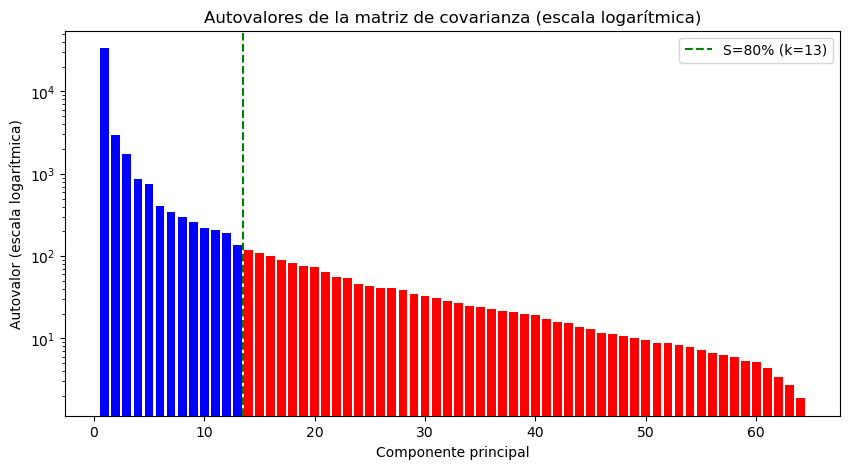
\includegraphics[width=1\textwidth]{Ejercicio3.png}
    \caption{Espectro de autovalores de la matriz de covarianza sobre bloques de $8\times 8$. Los componentes principales conservados (azul) corresponden a las direcciones de mayor varianza, mientras que los descartados (rojo) representan información redundante. La caída pronunciada evidencia que la mayor parte de la información se preserva utilizando un subconjunto reducido de componentes, como se predice en \eqref{eq:proyeccion}.}
    \label{fig:ej2}
\end{figure}

Como vemos en la Figura 3, el espectro de autovalores decrece rápidamente, lo que indica que la mayor parte de la varianza de los datos está concentrada en unas pocas componentes. Este comportamiento es consistente con la teoría de PCA, que busca identificar las direcciones de máxima varianza para reducir la dimensionalidad sin perder información relevante.

\subsection{Descompresión}

La reconstrucción de la imagen se realizó revirtiendo la proyección PCA\eqref{eq:reconstruccion}, utilizando los componentes principales conservados (Y , Vk, $\mu$). El resultado fue una imagen visualmente muy similar a la original, aunque con ligeras pérdidas en detalles finos y texturas, atribuibles a la eliminación de componentes de menor varianza. Este resultado práctico valida la capacidad de PCA para comprimir imágenes manteniendo la calidad visual, especialmente cuando la redundancia espacial es alta.

\begin{figure}[H]
    \centering
    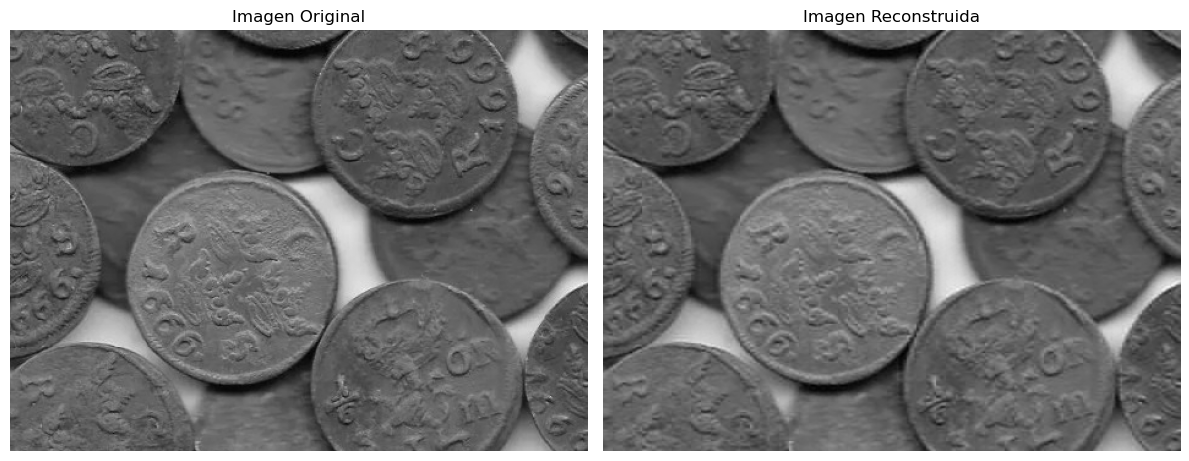
\includegraphics[width=\textwidth]{Ejercicio4.png}
    \caption{Comparación visual entre la imagen original (izquierda) y la reconstruida mediante PCA (derecha).}
    \label{fig:ej3}
\end{figure}

\subsection{Medidas de desempeño}

El desempeño de la compresión se evaluó mediante el error cuadrático medio (MSE) definido en \eqref{eq:mse} para distintos niveles de ahorro de espacio $S$, desde 5\% hasta 95\%. Los resultados muestran que el MSE aumenta de forma constante al incrementar $S$, es decir, al retener menos componentes principales. Este comportamiento es coherente con la teoría: al reducir la dimensionalidad, se descarta información y aumenta el error. Cabe señalar que, cómo se evaluó en la Sección 3.1, la relación entre el MSE y el porcentaje de compresión depende de las características particulares de la imagen analizada.

\begin{figure}[H]
    \centering
    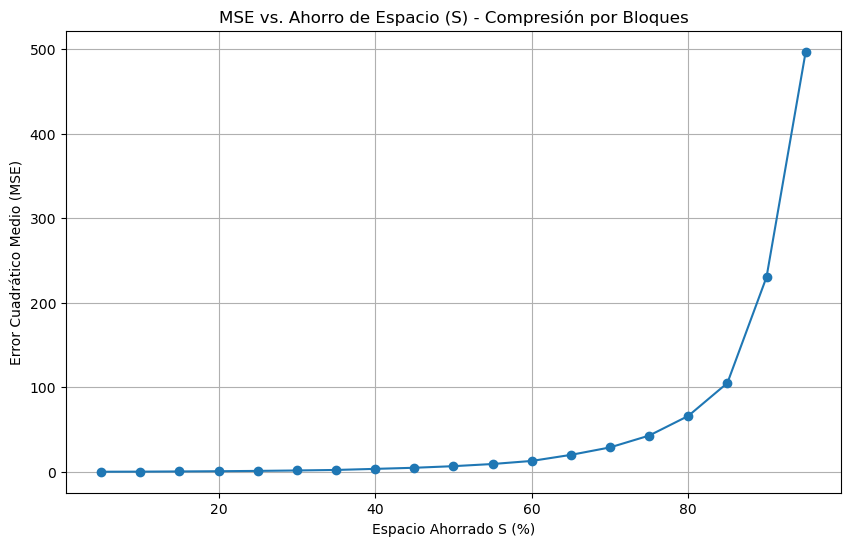
\includegraphics[width=0.8\textwidth]{Ejercicio5.png}
    \caption{Error cuadrático medio (MSE) de la reconstrucción en función del porcentaje de ahorro de espacio $S$. Se observa que al retener menos componentes principales, aumenta el error de reconstrucción, reflejando el compromiso entre compresión y calidad visual}
    \label{fig:mse}
\end{figure}

\begin{figure}[H]
    \centering
    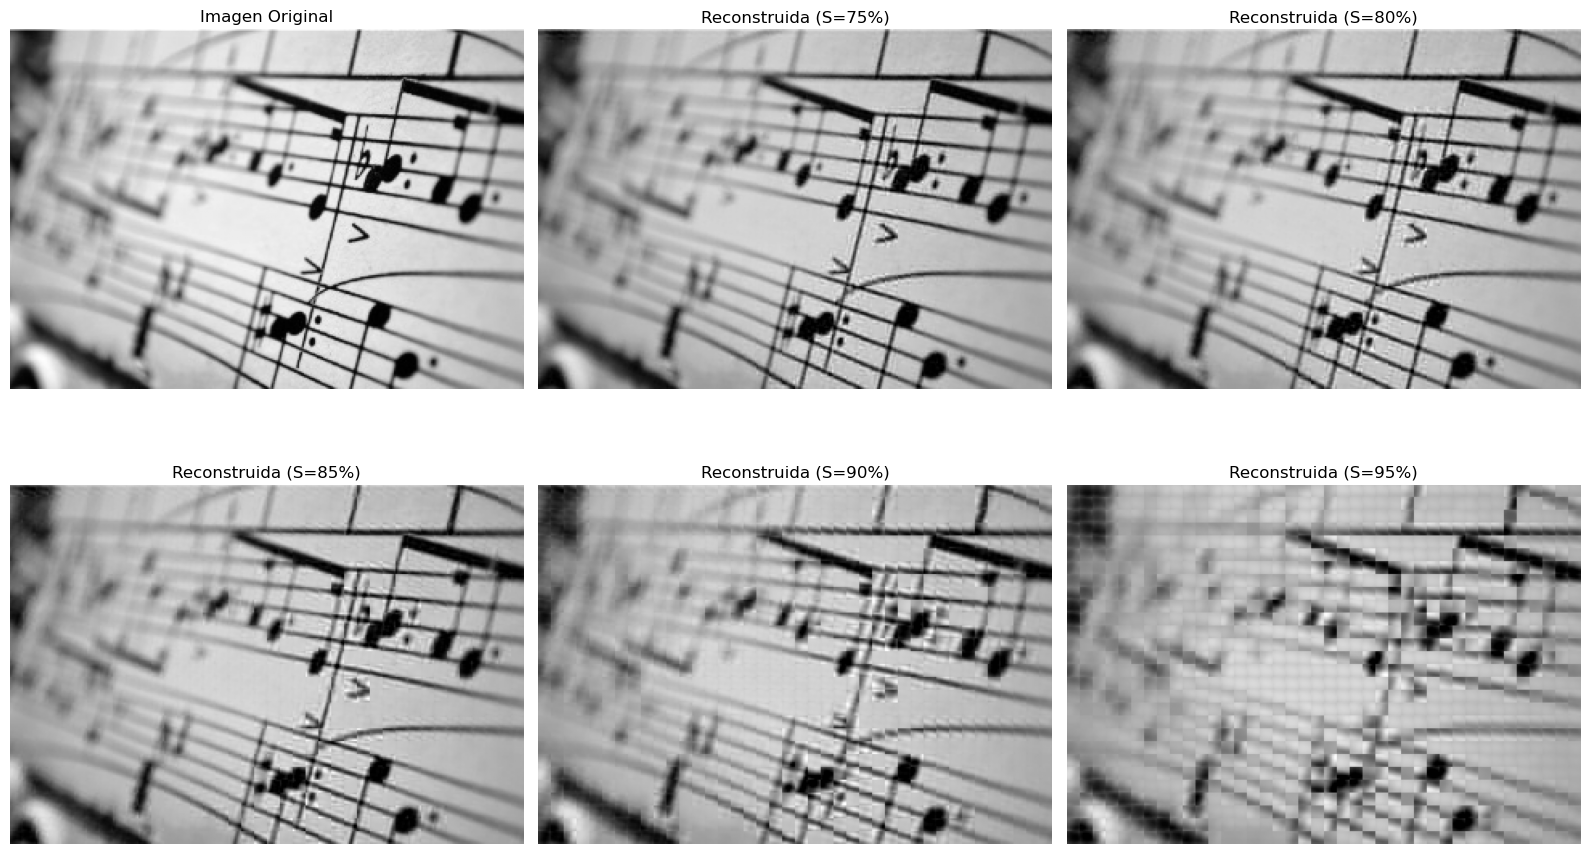
\includegraphics[width=0.8\textwidth]{Ejercicio6.png}
    \caption{Comparación entre la imagen original y su reconstrucción con $S=85\%$, $S=90\%$, $S=95\%$.}
    \label{fig:ej6}
\end{figure}

El análisis visual complementario evidenció una degradación progresiva de la calidad a medida que aumentaba el valor de $S$. No obstante, incluso con un 85\% de ahorro de espacio, la imagen conserva una estructura global fácilmente reconocible y las pérdidas de calidad se concentran principalmente en los detalles finos y la nitidez. Con $S=95\%$ la estructura general sigue siendo identificable, aunque la distorsión resulta ya notoria. Este comportamiento, si bien esperable en términos teóricos, resulta llamativo por la magnitud del ahorro de información logrado frente a la calidad aún preservada en la reconstrucción.

% ---------- CONCLUSIONES ----------
\section{Conclusiones}

Todo lo expuesto anteriormente demuestra el potencial del análisis de componentes principales (PCA) para reducir la dimensionalidad de las imágenes preservando la mayor cantidad posible de información. Este efecto resulta particularmente evidente cuando la correlación local entre píxeles es alta, ya que la redundancia de datos se traduce en una concentración del peso de la varianza en pocos autovalores. En consecuencia, es posible descartar una mayor cantidad de componentes sin generar pérdidas significativas, lo que refuerza la coherencia entre los resultados obtenidos y los fundamentos teóricos del método.

A continuación, se implementó el algoritmo de PCA desde cero, segmentando las imágenes en bloques y proyectando los datos en un subespacio de menor dimensión mediante una implementación propia de la descomposición en valores singulares (SVD). Durante este proceso, al comparar el rendimiento de nuestra función \texttt{our\_svd} con la función nativa de \texttt{NumPy} (\texttt{np.linalg.svd}), se observó la aparición de una distorsión en los resultados al emplear la segunda, lo que motivó un análisis más detallado de las diferencias entre ambas implementaciones.

\begin{figure}[H]
    \centering
    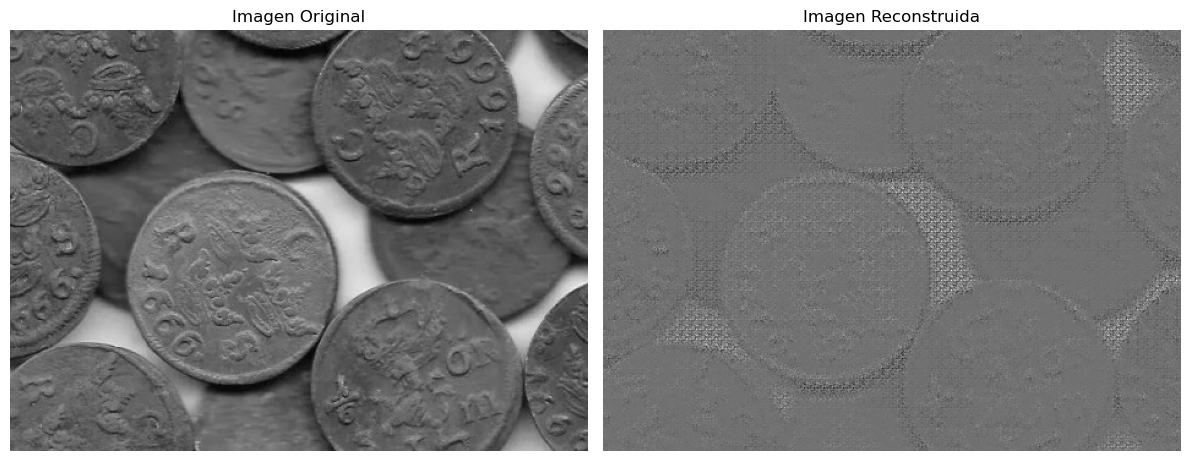
\includegraphics[width=\textwidth]{ErrorSVD.png}
    \caption{Comparación entre reconstrucciones obtenidas con nuestra implementación de SVD (\texttt{our\_svd}) y con \texttt{np.linalg.svd}. En este último caso se observaron distorsiones visuales, atribuibles a la ausencia de la transposición necesaria en el procedimiento de PCA.}
    \label{fig:svd}
\end{figure}

Esta diferencia se identificó tras una tarea de depuración, en la cual comprobamos que nuestra función \texttt{our\_svd} producía reconstrucciones correctas mientras que \texttt{np.linalg.svd} introducía distorsiones visibles. La causa radica en que \texttt{our\_svd} opera directamente sobre la matriz de covarianza, obteniendo autovalores y autovectores ya alineados con la formulación de PCA (ya que fue diseñada teniendo esto en mente), mientras que la función nativa de numpy realiza la descomposición sobre la matriz de datos original y devuelve la factorización estándar $U,S,V^T$. Aunque ambas aproximaciones son matemáticamente equivalentes, la salida de NumPy no está adaptada de manera inmediata para PCA: los vectores aparecen como $V^T$ en lugar de $V$, los signos pueden invertirse y los valores singulares requieren reinterpretarse para reflejar la varianza explicada. La falta de estos ajustes fue lo que generó las distorsiones, y la depuración realizada nos permitió concluir la importancia de controlar explícitamente la correspondencia entre autovalores, autovectores y valores singulares en la implementación del método.

Finalmente, este trabajo abre la puerta a posibles mejoras y extensiones. Una primera línea sería comparar el desempeño de PCA con otros métodos de compresión más utilizados en la práctica y evaluar sus rendimientos computacionales. También resultaría interesante analizar la sensibilidad del algoritmo frente a distintos tipos de imágenes (fotografías, texturas, patrones sintéticos) y estudiar cómo la correlación espacial afecta de manera diferencial la compresibilidad.

\end{document}